% =====================================================================
% Segunda parte – 6. Pruebas de aceptación
% =====================================================================
\section{Pruebas de aceptación}

\subsection{Organización de la prueba}

La prueba de aceptación la ejecuta un \textbf{usuario final} (\pendiente{nombre y perfil del usuario final}) sobre la aplicación \textbf{desplegada} (\url{https://shifts-chash-version-amaya.vercel.app/}), con una cuenta creada por él mismo durante la sesión (PA-10). Un integrante del equipo lee cada caso, no interviene en la ejecución y anota el resultado y las observaciones en el acta del Apéndice \ref{ap:acta}, que el usuario firma al final. Todos los casos se ejecutan por la interfaz, incluidos PA-03 y PA-05, que en la primera ejecución se hicieron por API.

Antes de la sesión, el equipo verificó los casos con el guion de Selenium (Apéndice \ref{ap:selenium}) en el ambiente local, para no exponer al usuario a defectos conocidos.

\subsection{Diseño de los casos de prueba}

{\footnotesize\renewcommand{\arraystretch}{1.15}
\begin{longtable}{L{1.1cm} L{1.3cm} L{3.2cm} L{4.6cm} L{3.2cm}}
\caption{Guion de los casos de prueba de aceptación}\label{tab:pa}\\
\toprule
ID & Req. & Escenario & Pasos y datos & Resultado esperado \\
\midrule
\endfirsthead
\toprule
ID & Req. & Escenario & Pasos y datos & Resultado esperado \\
\midrule
\endhead
\bottomrule
\endfoot
PA-01 & RNF04 & Ruta privada sin sesión & Abrir \codigo{/dashboard} sin haber iniciado sesión & Redirige a \codigo{/login} \\
PA-10 & RF01, RF02 & Registrarse e iniciar sesión & Crear una cuenta con correo y contraseña de 8+ caracteres; cerrar sesión; iniciar sesión (opcional: con Google) & Entra al dashboard con su nombre \\
PA-02 & RF03, RF08 & Registrar un gasto & «+ Transacción»: gasto de 45\,000 en Alimentación, «Almuerzo» & Aparece en el historial y el total gastado sube 45\,000 \\
PA-03 & RF04 & Ingreso recurrente & Ingreso de 2\,500\,000, Salario, recurrente mensual & Queda marcado como recurrente (ícono en el historial) \\
PA-04 & RF04 & Recurrente sin frecuencia & Activar «recurrente» sin elegir frecuencia y guardar & No se guarda y se pide la frecuencia \\
PA-11 & RF06 & Editar y eliminar una transacción & Abrir el detalle de «Almuerzo», cambiar el monto a 40\,000; luego eliminarla & El cambio se refleja; al eliminarla desaparece y el total baja \\
PA-12 & RF07 & Filtrar el historial & Buscar «Almuerzo»; filtrar por tipo gasto y por fechas & Solo se ven las transacciones que cumplen el filtro \\
PA-16 & RF10 & Gestionar categorías & Crear la categoría «Mascotas»; registrar un gasto en ella; intentar eliminarla & Se crea; al eliminarla con transacciones aparece un mensaje que lo impide \\
PA-05 & RF11 & Crear un presupuesto & Presupuesto «Comida del mes», Alimentación, 600\,000, mensual del mes actual & Aparece la tarjeta con el gasto ya registrado \\
PA-06 & RF12 & Presupuesto superado & Registrar gastos de Alimentación hasta superar 600\,000 & La tarjeta muestra el porcentaje real ($> 100$\,\%) en rojo \\
PA-17 & RF13, RF18 & Editar presupuesto y meta & Cambiar el monto del presupuesto; cambiar la fecha final de una meta & Se recalculan el porcentaje y el plan \\
PA-14 & RF14 & Alerta de umbral & Con el umbral en 80\,\%, superar el 80\,\% del presupuesto total & El resumen muestra la alerta \\
PA-07 & RF15, RF16 & Crear una meta & Meta de 1\,000 con fin en 14 días & 15 casilleros, ninguno negativo; suma 1\,000 \\
PA-08 & RF15 & Monto no redondo & Meta de 1\,500 & Mensaje «El monto debe ser un número redondo (múltiplo de 1000)» \\
PA-09 & RF17 & Marcar días & Marcar los días 1 a 3 y «Guardar días» & «Guardado» y porcentaje actualizado \\
PA-13 & RF09 & Ver gráficas & Abrir Gráficas y cambiar el período & Los totales coinciden con el resumen \\
PA-15 & RF19, RF20 & Perfil y tema & Cambiar el nombre, la moneda y el tema; recargar & Los cambios se conservan \\
\end{longtable}
}
\vspace{-1em}
{\small\textit{Nota.} RF05 (generación automática de recurrentes) no es observable en una sesión de una hora; se acepta con la evidencia de PI-08 y verificando al día siguiente la instancia del ingreso de PA-03. Los casos PA-10 a PA-17 son nuevos. Fuente: elaboración propia.}

\subsection{Verificación previa del equipo}

\begin{table}[H]
\caption{Resultados de la verificación previa (sin usuario final)}
\label{tab:pa-previo}
\footnotesize
\begin{tabularx}{\linewidth}{L{1.2cm} Y Y}
\toprule
ID & 25/10/2026 (commit \codigo{0efe28b}) & 21/11/2026 (rama \codigo{fix/defectos}) \\
\midrule
PA-01 & Aprobado & Aprobado (Selenium) \\
PA-02 & Aprobado & Aprobado (Selenium) \\
PA-03 & Aprobado solo por API & Aprobado por la interfaz (Selenium): el ingreso queda marcado como recurrente \\
PA-04 & Aprobado parcial: el envío se bloquea con el mensaje nativo del navegador & Sin cambios (observación aceptada) \\
PA-05 & Aprobado solo por API & Aprobado por la interfaz (Selenium): aparece la tarjeta del presupuesto \\
PA-06 & \textbf{Fallido}: 100\,\% en lugar de 117\,\% (D-04) & Aprobado: muestra 124\,\% en rojo (Selenium, Figura \ref{fig:pa06-despues}) \\
PA-07 & \textbf{Fallido}: el día 15 muestra $-400$ (D-01) & Aprobado: 10 cuotas de 100 y 5 de 0 (Figura \ref{fig:p-reto}) \\
PA-08 & Aprobado & Aprobado (Selenium) \\
PA-09 & Aprobado & Aprobado (PI-06 y prueba manual) \\
\bottomrule
\end{tabularx}
\tablenote{Ejecutado en el ambiente local con datos ficticios. Fuente: elaboración propia.}
\end{table}

\begin{minted}[fontsize=\footnotesize, frame=single]{text}
$ SC_BASE_URL=http://127.0.0.1:5173 SC_HEADLESS=1 python tests/aceptacion_selenium.py
PA-01 OK
PA-02 OK
PA-03 OK
PA-05 OK
PA-06 captura guardada
PA-08 OK
\end{minted}

\begin{figure}[H]
\centering
\caption{PA-06 en la segunda ejecución: presupuesto superado con el porcentaje real}
\label{fig:pa06-despues}
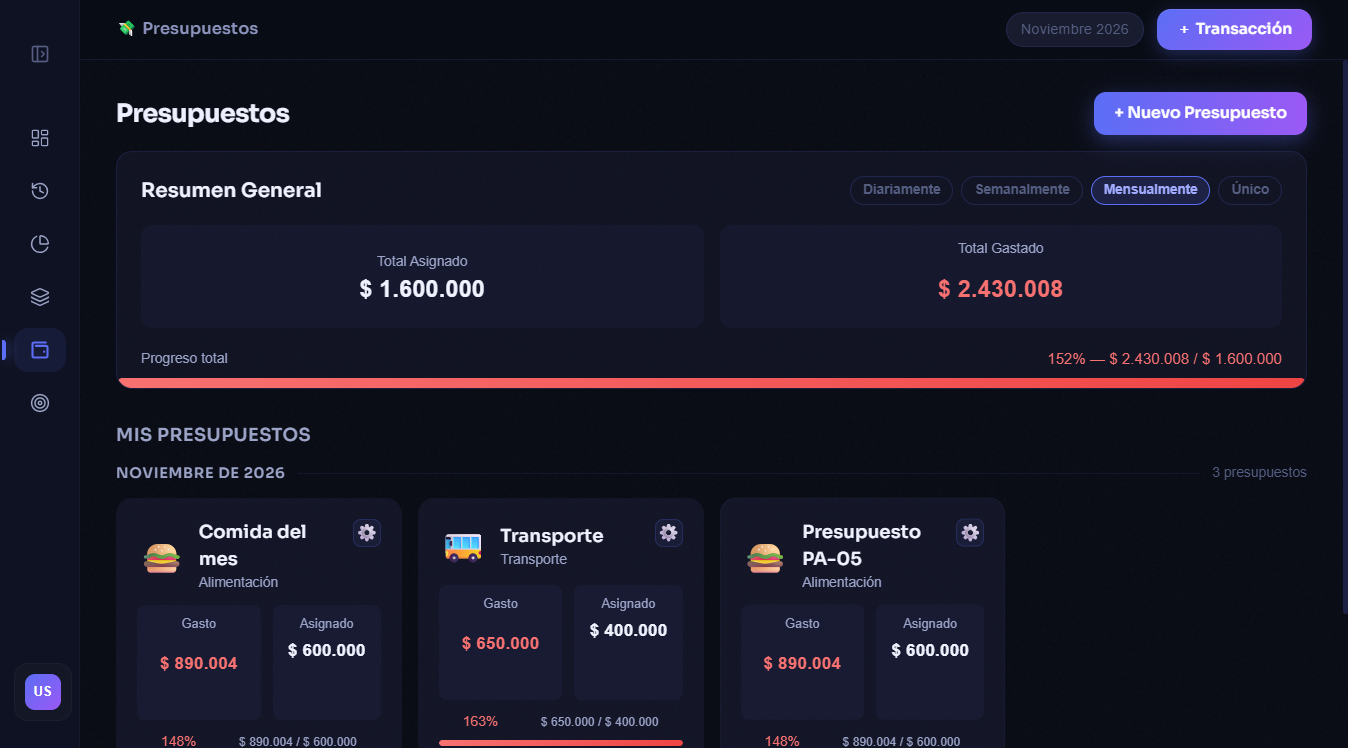
\includegraphics[width=0.8\linewidth]{../evidencias/pa06_presupuestos.png}
\figurenote{Captura de Selenium. Fuente: elaboración propia.}
\end{figure}

\begin{figure}[H]
\centering
\caption{PA-07 en la primera ejecución: cuota negativa del día 15 (D-01)}
\label{fig:pa07-antes}
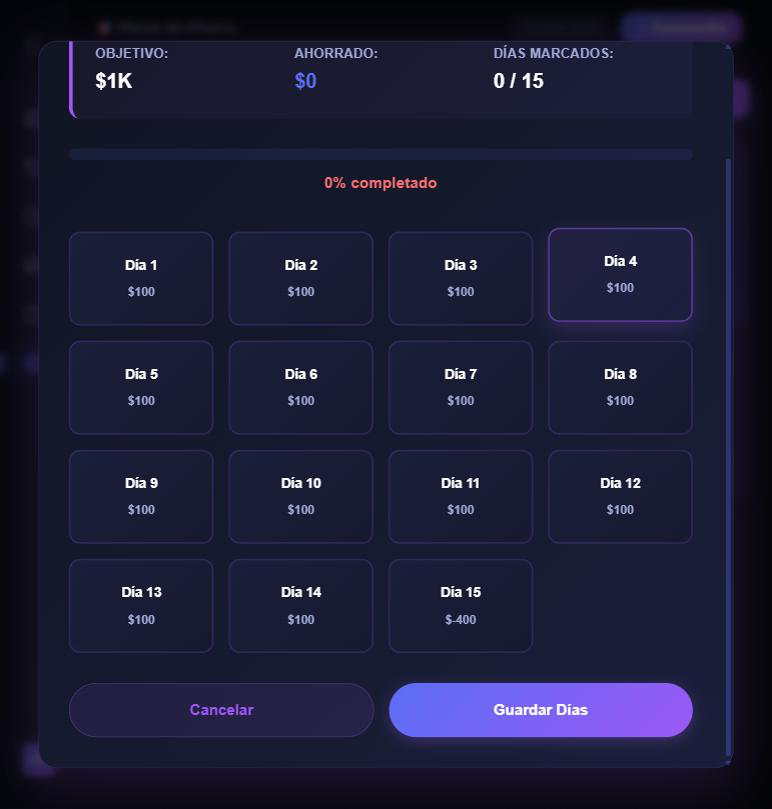
\includegraphics[width=0.7\linewidth, height=0.35\textheight, keepaspectratio]{previo/pa07_antes_cuota_negativa.png}
\figurenote{Fuente: elaboración propia.}
\end{figure}

\subsection{Ejecución y evaluación con el usuario final}

\begin{table}[H]
\caption{Evaluación de la prueba de aceptación}
\label{tab:eval-aceptacion}
\footnotesize
\begin{tabularx}{\linewidth}{L{3.6cm} Y}
\toprule
Aspecto & Resultado \\
\midrule
Usuario y fecha & \pendiente{nombre, perfil y fecha de la sesión} \\
Ambiente & Aplicación desplegada en Vercel y Render, versión \pendiente{commit desplegado} \\
Casos ejecutados & \pendiente{número de casos ejecutados de 17} \\
Casos aceptados / rechazados & \pendiente{aceptados y rechazados} \\
RF aceptados & \pendiente{RF aceptados de 20 y porcentaje (objetivo $\geq 90$\,\%)} \\
Observaciones del usuario & \pendiente{observaciones textuales del acta} \\
Acciones & \pendiente{acción por cada observación: corrección, mejora futura o aceptada} \\
Concepto final & \pendiente{aceptado, aceptado con observaciones o rechazado} \\
Evidencia & Acta firmada (Apéndice \ref{ap:acta}): \pendiente{escaneo del acta firmada} \\
\bottomrule
\end{tabularx}
\tablenote{Fuente: elaboración propia.}
\end{table}

\paragraph{Cálculo del porcentaje de RF aceptados.} Un RF se acepta si todos los casos que lo cubren en la Tabla \ref{tab:pa} se aceptan. El porcentaje es $\frac{\text{RF aceptados}}{20} \times 100$.
